\chapter{Future work}

\label{ch:future}

\section{Fission product empirical potential}

In order to study the interaction of fission products with larger features in the cladding microstructure, such as dislocations and grain boundaries, it is necessary to develop empirical potentials for use in molecular dynamics simulations. Grain boundary transport is of particular interest, and this would require something on the order of 10$^{4}$ atoms to simulate to a reasonable degree of accuracy. This cannot be done using DFT currently due to the significant amount of computing resources required to run such a simulation. 

The development of an iodine and xenon potential with \zirconia\ should be prioritised in order to run simulations to determine the migration of iodine within \zirconia, followed by the behaviour of xenon at the equilibrium iodine sites.

\section{Grain boundary transport}

Grain boundaries are interesting areas for studying species migration because diffusion towards the metal is expected to be more rapid through them than through bulk \zirconia .

\section{Zr/ZrO/\zirconia\ interface study}

The inner oxide is not a homogeneous structure, as described in § \ref{ch:crystallography}. Figure \ref{fig:zro_interface} clearly shows the existence of a ZrO phase up to 200 nm thick at the interface between \zirconia\ and Zr metal. The presence of ZrO and even oxygen-saturated Zr metal will have an effect on the thermodynamic equilibria of different fission products. An interface study can be conducted using DFT, to determine stresses at the interfaces of Zr and ZrO, and ZrO and \zirconia . Studying the aggregate effect of these interfaces on fission product behaviour may require larger molecular dynamics simulations, however. The crystal structure of the ZrO phase has been studied using both simulation and high-resolution electron microscopy, with two likely crystal structures being proposed \cite{Nicholls2015}. Further atomistic studies must be conducted to determine the stability of each crystal structure of ZrO when constrained by \zirconia\ and oxygen-saturated Zr metal interfaces.


\begin{figure}
    \centering
    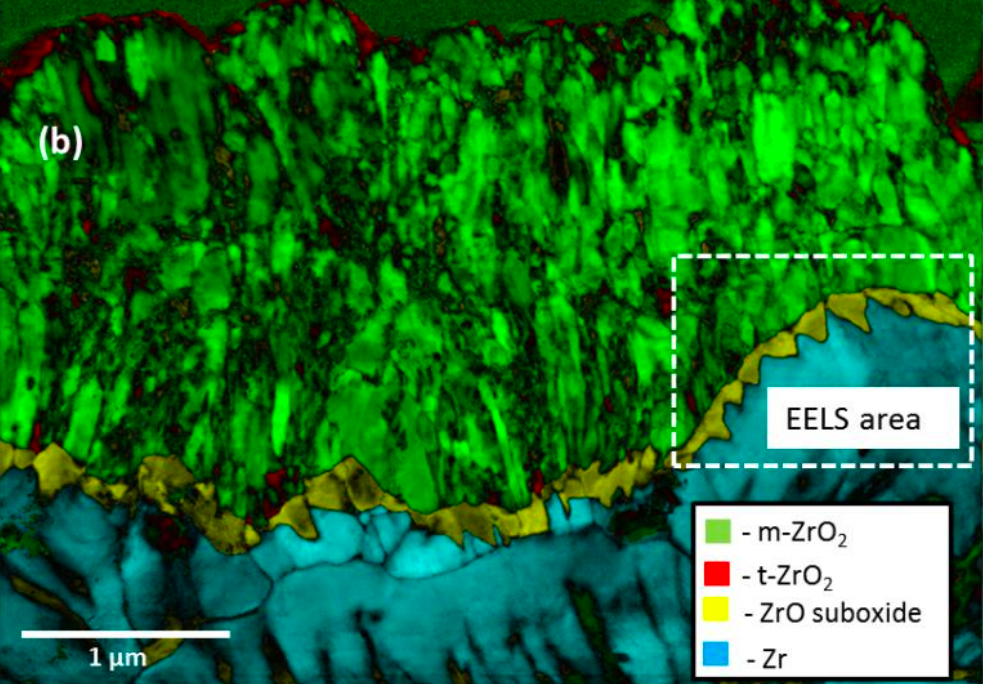
\includegraphics[height=9cm]{images/zro_interface.png}
    \caption[STEM image of a Zr-1.0\%Nb sample oxidised in simulated PWR water at 360 C for 120 days.]{STEM image of a Zr-1.0\%Nb sample oxidised in simulated PWR water at 360 C for 120 days. Taken from \cite{inproceedings}.}
    \label{fig:zro_interface}
\end{figure}